\documentclass[xcolor=pdftex,dvipsnames,table,mathserif,aspectratio=169]{beamer}
\usetheme{metropolis}
%\usetheme{Darmstadt}
%\usepackage{times}
%\usefonttheme{structurebold}

\usepackage[english]{babel}
%\usepackage[table]{xcolor}
\usepackage{pgf,pgfarrows,pgfnodes,pgfautomata,pgfheaps}
\usepackage{amsmath,amssymb,setspace,centernot}
\usepackage[latin1]{inputenc}
\usepackage[T1]{fontenc}
\usepackage{relsize}
\usepackage{pdfpages}
\usepackage[absolute,overlay]{textpos} 

\DeclareMathSizes{10}{10}{6}{6} 


\title [Dynamic Demand I]{Dynamic Demand I:\\
 Durable Goods + Storable Goods}
\author{C.Conlon}
\institute{Grad IO}
\date{\today}
\setbeamerfont{equation}{size=\tiny}
\begin{document}

\begin{frame}
\titlepage
\end{frame}

\begin{frame}{Today's Readings}
\begin{itemize}
\item Melnikov (Yale PhD Thesis 2001)
\item Gowrisankaran Rysman (JPE)
\item Hendel and Nevo (Econometrica )

\end{itemize}
\end{frame}


\begin{frame}{Dynamic Demand}
\begin{itemize}
\item Earlier this term we looked at \textit{static models of product differentiation} such as BLP (1995).
\item We have also looked at single agent models of dynamic behavior such as Rust (1987).
\item What if we could put those two together? Why?
\end{itemize}
\end{frame}

\begin{frame}{Two Examples}
\begin{itemize}
\item Durable Goods
\begin{itemize}
\item We are often interested in the case where a firms' products compete not only against products of other firms, but also with their own products over time. (Coase 1972).
\item Really this is a feature of any kind of durable (cars, washing machines, etc.).
\item In high-tech products, we have `S'-shaped penetration curve. At some point we cut the prices of (computers, cameras, TV's) and the sales go down rather than up. Why?
\item Static estimates imply demand is \alert{less elastic} than it really is.
\end{itemize}
\item Storable Goods
\begin{itemize}
\item Laundry detergent goes on discount: $\approx$ 1 week in every 4-8.
\item A large fraction of overall quantity is sold during these discount weeks.
\item This would imply highly elastic demand. (1) Laundry detergent business must be extremely competitive. (2) There would be a substantial response to a \alert{permanent} price change. Seems unlikely that (1) and (2) are true.
\item Static estimates imply demand is \alert{more elastic} than it really is.
\end{itemize}
\end{itemize}
\end{frame}

\begin{frame}{Dynamic Demand  (Gowrisankaran Rysman)}
\begin{figure}[htbp]
\begin{center}
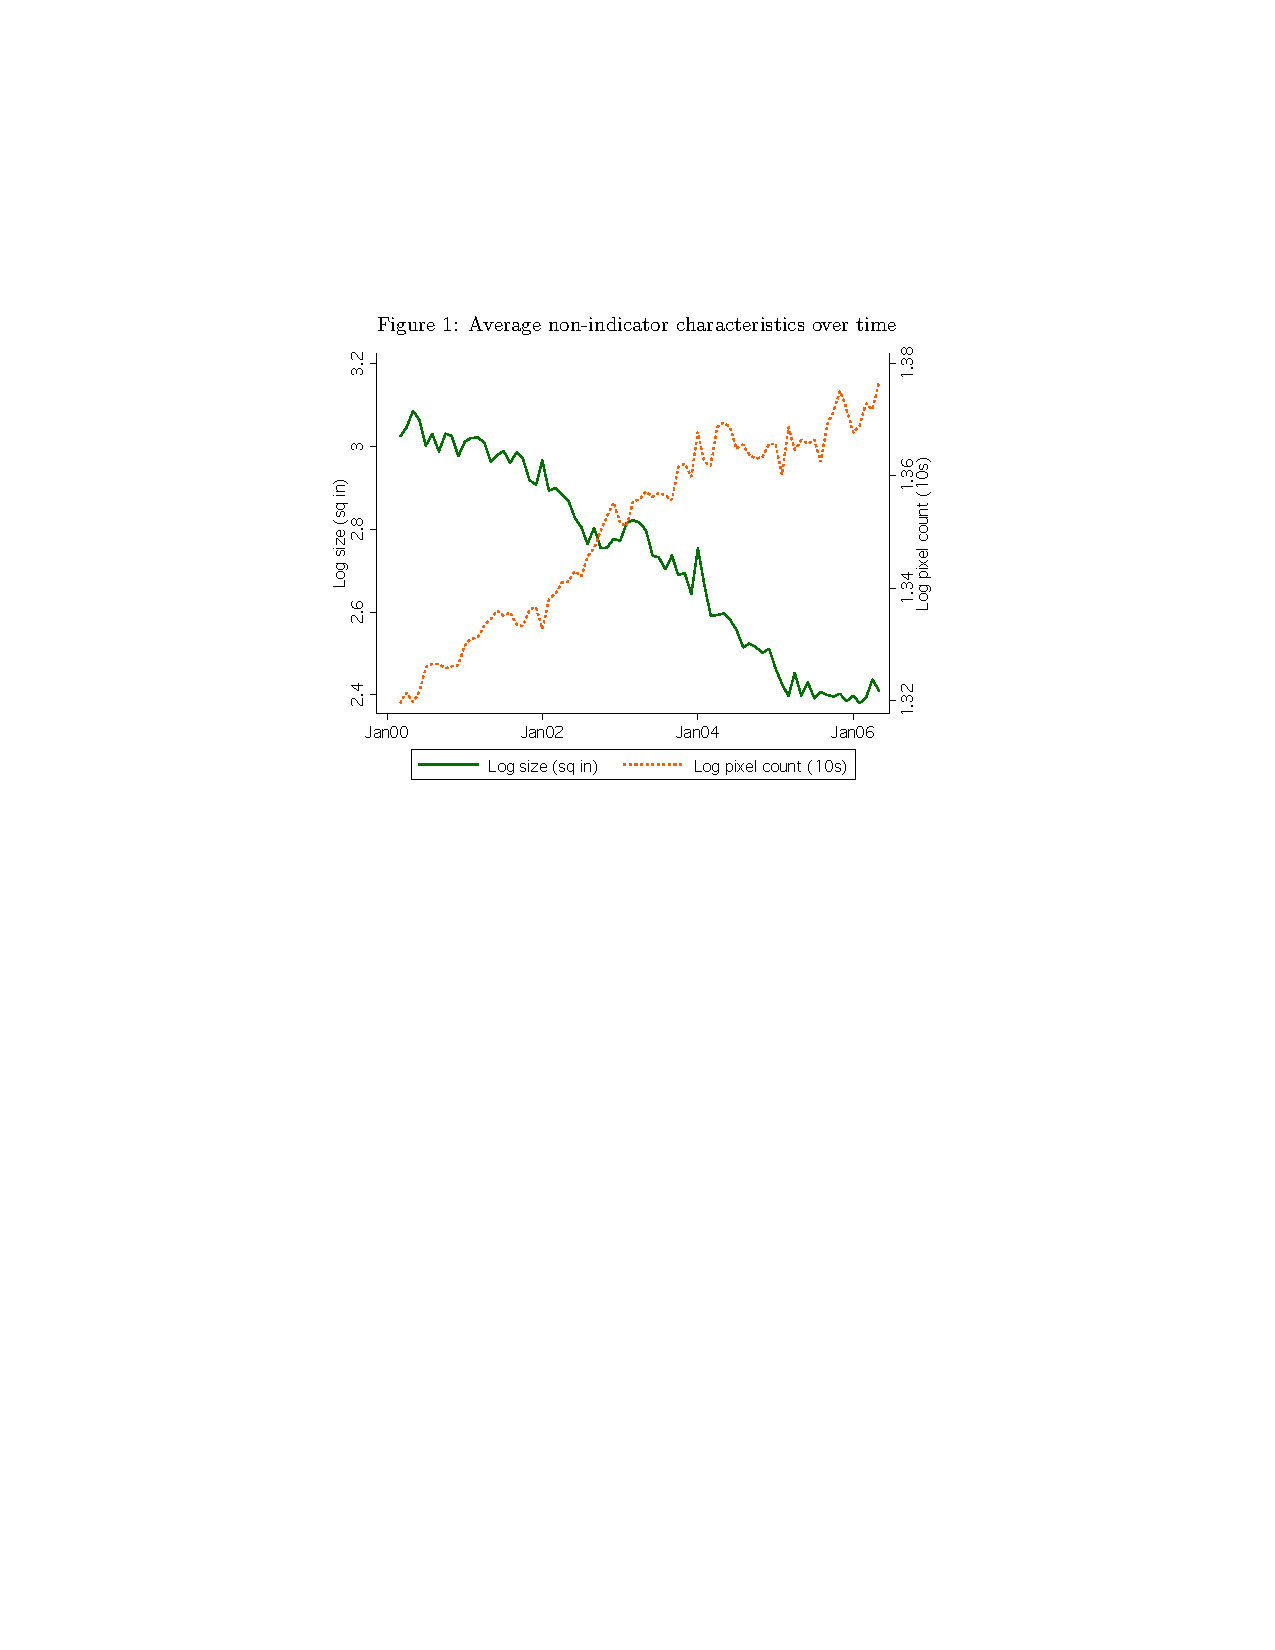
\includegraphics[width=4in]{resources/gandr1.pdf}
\label{gandr1}
\end{center}
\end{figure}
\end{frame}

\begin{frame}{Dynamic Demand (Gowrisankaran Rysman)}
\begin{figure}[htbp]
\begin{center}
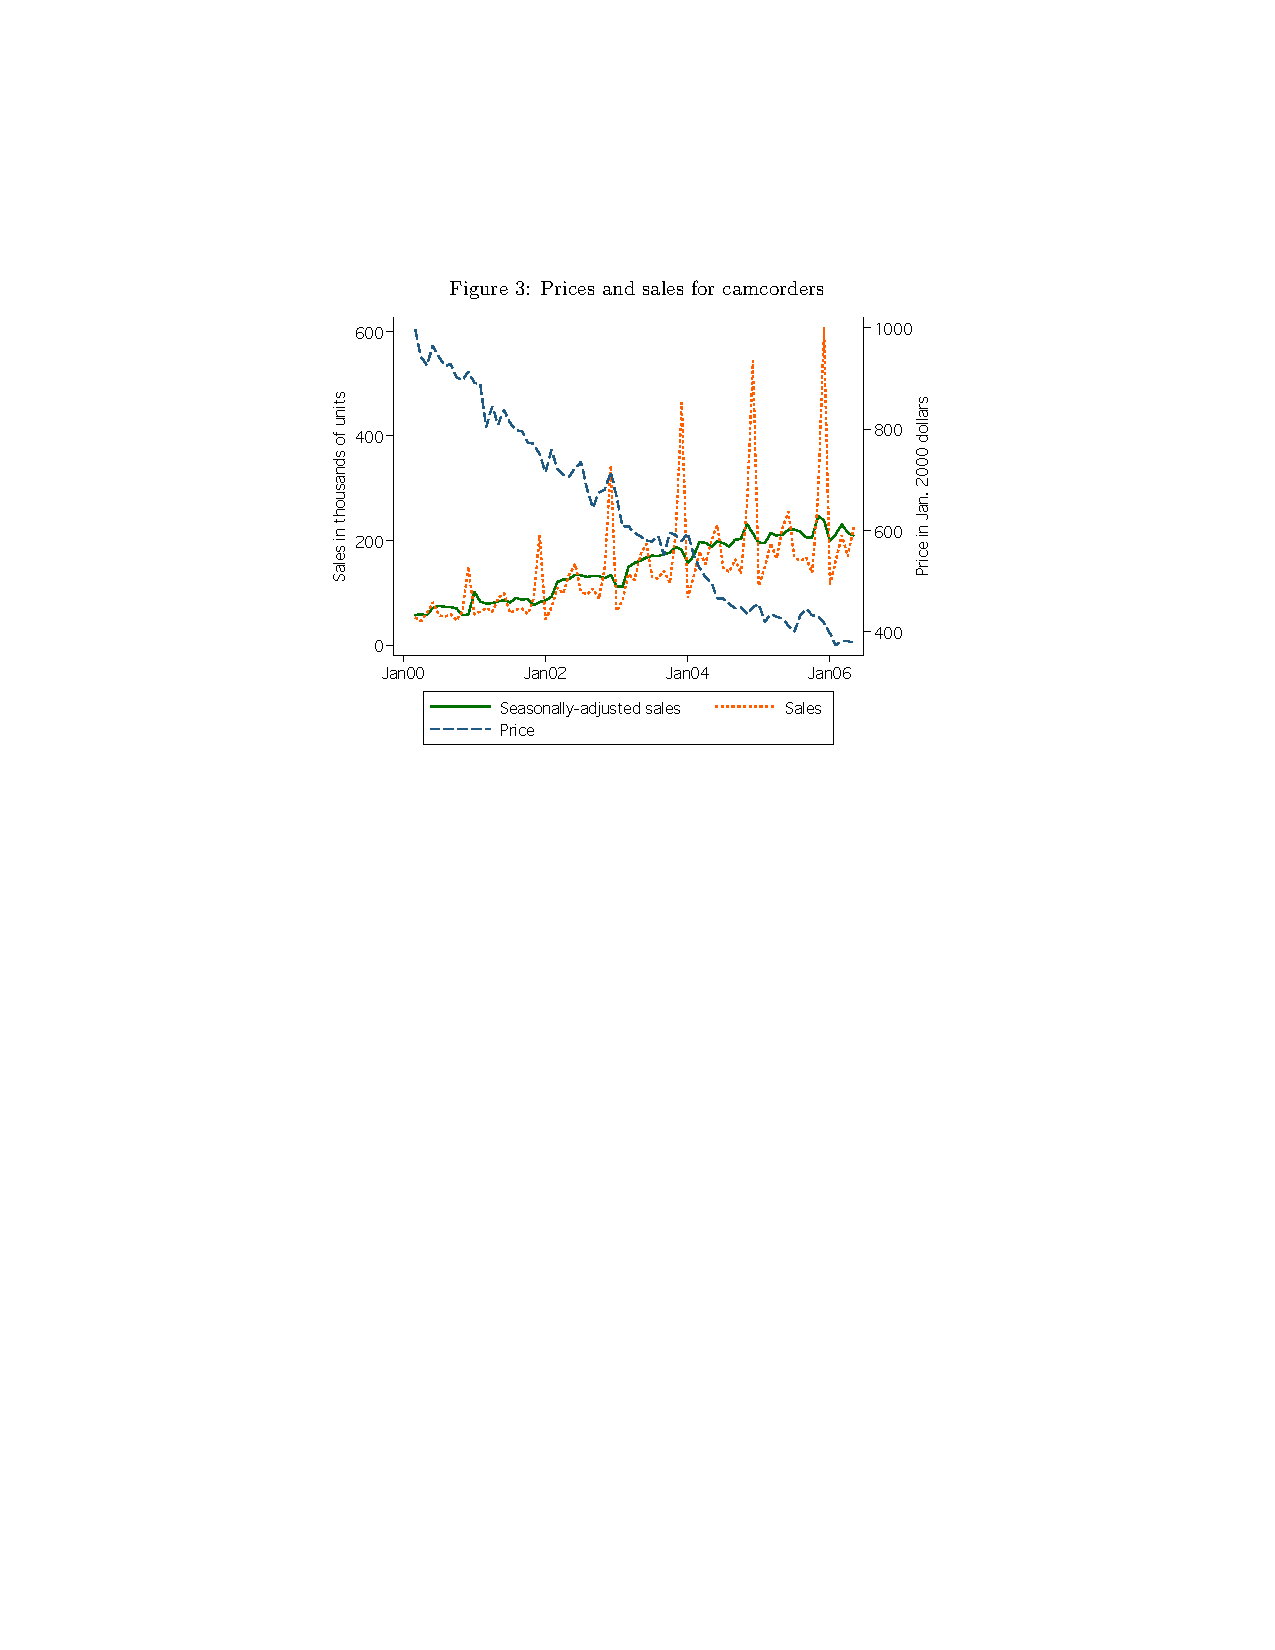
\includegraphics[width=4in]{resources/gandr2.pdf}
\label{gandr2}
\end{center}
\end{figure}
\end{frame}

\begin{frame}{Dynamic Demand (Gowrisankaran Rysman)}
Imagine if we regressed $P$ on $Q$:
\begin{itemize}
\item In early periods $P$ falls and $Q$ rises.
\item In later periods $P$ falls and $Q$ also falls (top of the $S$-curve).
\item Depending on the time period we might find that demand slopes \alert{upwards} (lower prices lead to lower sales)
\end{itemize}
\end{frame}



%\begin{frame}{Dynamic Demand}
%\begin{figure}[htbp]
%\begin{center}
%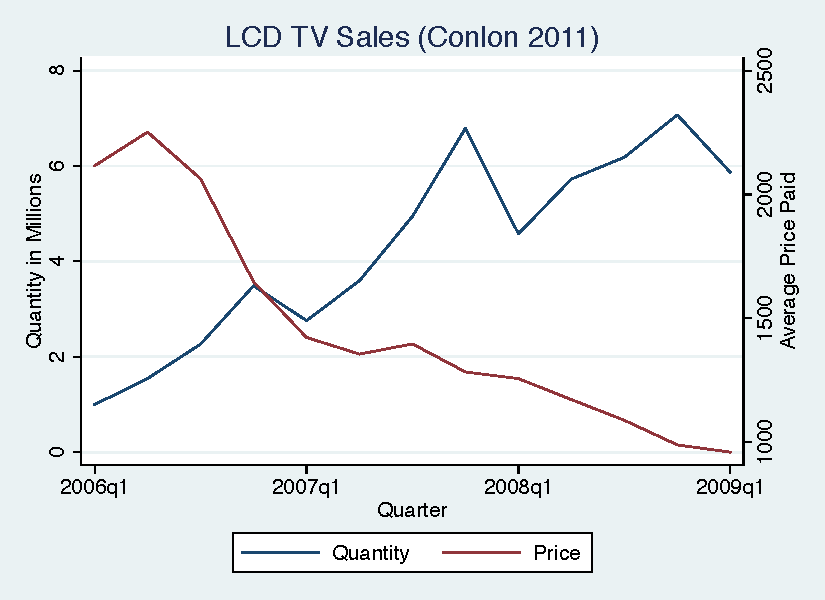
\includegraphics[width=4in]{resources/conlon1.pdf}
%\label{conlon1}
%\end{center}
%\end{figure}
%\end{frame}
%
%\begin{frame}{Dynamic Demand}
%\begin{figure}[htbp]
%\begin{center}
%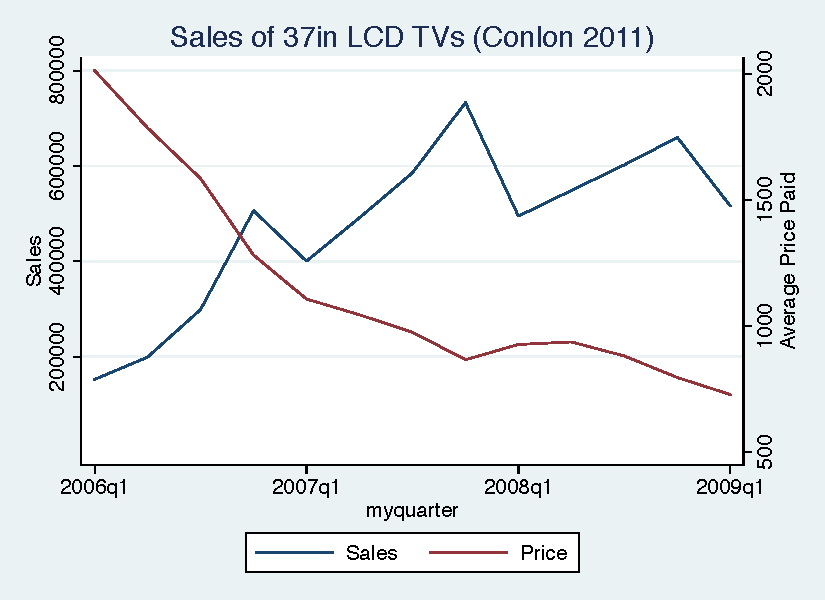
\includegraphics[width=4in]{resources/conlon2.pdf}
%\label{conlon1}
%\end{center}
%\end{figure}
%\end{frame}

\begin{frame}{Dynamic Demand}
\begin{itemize}
\item Today a 55" 4K LCD TV is \$400. In 2006, you could buy a 32" 720P TV for $>\$10,000$.
\item In December 2011 TV prices fell $17\%$ on an annual basis and other A/V equipment fell $11\%$, and computer equipment fell $14\%$.
%\item Conlon 2016 reports a 22\% annualized price decline in LCD TV's from 2006-2009.
\item From August 2005 to August 2015 prices declined by 87.2\%.
\item We might also find that over time consumers buy better cameras or larger TV's
\item The BLS tries to do \textit{chaining} and \textit{quality adjustments} but in high-tech products this can be very difficult.
\item This has a potentially large impact on price indices (a small bias in the CPI can be billions of dollars in SSA/Medicare payments).
\end{itemize}
\end{frame}



\begin{frame}{Dynamic Demand: Stripped Down Version}
Let's start with some very strong assumptions to get our intuition clear:
\begin{enumerate}
\item There are $t=1,2$ periods.
\item Consumers can purchase at most one unit of an (infinitely) durable good
\item After purchasing the durable good they leave the market forever.
\end{enumerate}
\end{frame}

\begin{frame}{Dynamic Demand: Naive Static Approach}
\begin{align*}
u_{ijt} &=   \alpha_i x_{jt}  +  \xi_{jt} + \varepsilon_{ijt}\\
u_{i0t} &=  \varepsilon_{i0t} 
\end{align*}
\begin{itemize}
\item Suppose  we estimate demand treating each period $t=1,2$ as a \alert{separate market}.
\item ie: close our eyes and do BLP.
\item What do we get wrong? \pause
\begin{itemize}
\item How does $\frac{\partial q_{j,t}}{\partial p_{k,s}}$ look? How should it look?
\end{itemize}
\item Two problems: 
\begin{itemize}
\item period $t=1$ and $t=2$ are \alert{substitutes}
\item distribution of $f(\alpha_{it})$ is likely different in $t=1,2$.
\end{itemize}
\end{itemize}
\end{frame}


\begin{frame}{Dynamic Demand: Complete Information}
Suppose consumers have full information about all shocks $(x_{j1},x_{j2},\xi_{j1},\xi_{j2},\varepsilon_{ij1},\varepsilon_{ij2})$ in both periods. 
\begin{align*}
u_{ijt} &=   \alpha_i x_{jt}  +  \xi_{jt} + \varepsilon_{ijt}
\end{align*}
What would we do?
\begin{itemize}
\item Why not estimate static demand among $\bigcup_{t=1,2}  \mathcal{J}_t $ alternatives?
\item Remaining issues:
\begin{itemize}
\item Buying in period 1 allows me an additional period of consumption
\item Need to discount period 2 utility $\beta \times ( \alpha_i x_{jt}  +  \xi_{jt} + \varepsilon_{ijt})$ or $\beta \times ( \alpha_i x_{jt}  +  \xi_{jt} )+\varepsilon_{ijt}$
\item A single outside good of not purchasing in either period $ u_{i0} =  \varepsilon_{i0} $
\end{itemize}
\item How bad is this model? Compared to the last one?
\end{itemize}
\end{frame}

\begin{frame}{Dynamic Demand: Relaxing some assumptions}
Problematic assumption was probably full information. Suppose instead that only $(\varepsilon_{ij2},\varepsilon_{i0})$ are \alert{unobserved} in $t=1$. 
\begin{align*}
v_{i0,t=1} \equiv E [\max_j u_{ij2}  | \Omega_{t=1}] = \log \left( \sum_j \exp [ \alpha_i x_{j2}  +  \xi_{j2} ] \right) + \eta
\end{align*}
\begin{itemize}
\item $\Omega_{t=1}= \{x_{j1},x_{j2},\xi_{j1},\xi_{j2},\varepsilon_{ij1}\}$ (everything known at $t=1$) 
\item $\eta$ is Euler's constant (per usual).
\item What about outside good?
\begin{itemize}
\item Either just another good in $t=2$ with $\alpha_i x_{j2}+ \xi_{j2} = 0$
\item Or we consider $v_{i0,t=1}=E [\max \{ \varepsilon_{i0}, \max_j u_{ij2} \}  | \Omega_{t=1}]$
\end{itemize}
\end{itemize}
\end{frame}

\begin{frame}{Dynamic Demand: Relaxing some assumptions}
Now what?
\begin{align*}
u_{ij,t=1} &=   \alpha_i x_{j1}  +  \xi_{j1} + \varepsilon_{ij1}\\
u_{i0,t=1} &=   \alert{\beta v_{i0,t=1}} + \varepsilon_{i01} \\
u_{ij,t=2} &=   \alpha_i x_{j2}  +  \xi_{j2} + \varepsilon_{ij2}\\
u_{ij,t=2} &=    \underbrace{\beta v_{i0,t=2} }_{=0}+ \varepsilon_{i02} 
\end{align*}
\begin{itemize}
\item If $\beta v_{i0,t=1}$ is known we can estimate static demand with each $t$ as a separate ``market''.
\item I pulled an extra $\varepsilon_{i01}$ out of my hat.
\item What is the other dynamic linkage?
\end{itemize}
\end{frame}


\begin{frame}{Dynamic Demand: What about cream skimming?}
Also need to account for the fact that $f(\alpha_{i,t=1})$ and $f(\alpha_{i,t=2})$  are not the same:
\begin{itemize}
\item If goods are perfectly durable, and consumers permanently exit the market...
\item Assume that $f(\alpha_{i,t=1}) = w_{i,t=1}$ is a discrete distribution of ``types''
\begin{itemize}
\item Note: ``type'' does not include $\varepsilon$.
\item then $w_{i,t=2} = w_{i,t=1} \cdot s_{i0,t=1}$
\end{itemize}
\end{itemize}
\end{frame}


\begin{frame}{Dynamic Demand: Can we go further?}
Replacement / Upgrades:
\begin{itemize}
\item Suppose we allow the people who purchase in $t=1$ to remain in the market.
\item Instead of comparing $u_{ij2}$ to $0$ they compare $u_{ij2}$ to their purchase in $t=1$.
\begin{itemize}
\item Now part of your ``type'' $\alpha_i$ includes your existing stock of the durable good.
\item Essentially increase the value of outside good.
\item The transitions become more complicated $w_{t=2} = f(w_{t=1},s_{ij,t=1})$.
\end{itemize}
\item You still throw the old durable into the trash when you are done.
\begin{itemize}
\item Could also allow for a scrap value.
\end{itemize}
\item Need to be a bit careful about NPV of expected stream of payments vs. ``flow utility'' now.
\end{itemize}
\end{frame}

\begin{frame}{Dynamic Demand: What about Beliefs?}
\begin{align*}
v_{i0,t=1} \equiv E [\max_j u_{ij2}  | \Omega_{t=1}] = \log \left( \sum_j \exp [ \alpha_i x_{j2}  +  \xi_{j2} ] \right) + \eta
\end{align*}

\begin{itemize}
\item This assumed that $x_{j2}$ and $\xi_{j2}$ were observed in $\Omega_{t=1}$.
\item Maybe we want to make some component of $x_{j2}$ \alert{unobserved} (such as price or $\xi$).
$$
\log \left( \sum_j \exp [ \alpha_i x_{j2}  +  \xi_{j2} ] \right)  g(p_2) 
$$
\item What do rational expectations mean here? More on this later.
\end{itemize}
\end{frame}




\begin{frame}{Dynamic Demand}
Each consumer type is subscripted by $i$, and chooses a product $j$ in period $t$ to maximize utility:
\begin{eqnarray*}
u_{ijt} &=&   \underbrace{\alpha_i^x x_{jt} +  \xi_{jt}}_{f_{jt}} - \alpha_{i}^p p_{jt} + \varepsilon_{ijt} \\
 u_{i0t} &=&  f_{i0t} + \varepsilon_{i0t} 
\end{eqnarray*}
In the static model we have $f_{i0t} = 0$ for every $i,t$.\\
\begin{itemize}
\item Where does the bias arise from?
\item Correlation between $f_{i0t}$ and prices.
\end{itemize}
\vspace{0.5cm}
We can think about dynamic models as having time varying utility for the outside option $f_{i0t}$
\begin{itemize}
\item What kind of good do I own now?
\item What do I anticipate in the future? (prices and quality)
\end{itemize}
\end{frame}

\begin{frame}{Dynamic Demand: Hypothetical}
\begin{itemize}
\item Suppose that I knew $f_{i0t}$ (falls from the sky).
\item Now we are back in the static logit world.
\item In fact, everything is consistent
\end{itemize}
\alert{Ad-Hoc approach:}
\begin{itemize}
\item  Just proxy with a time trend or sieve (Lou Prentice Ying 2012), (Eizenberg 2011) etc.  That is $f_{i0t} = \gamma_{0i} + \gamma_{1i} t + \gamma_{2i} t^2 + \ldots$
\item We can get the elasticity correct.
\item Not structural! Not helpful if we want to do counterfactuals! Can't get the elasticities under different conditions.
\item Is $f_{i0t}$ about current durable value? or Equilibrium beliefs about the future? (both!)
\end{itemize}
\end{frame}

\begin{frame}
\frametitle{Outside Good}
Goal is to endogenize the utility of the outside option $f_{i0t}$ using the model itself:
\begin{itemize}
\item Previous choice(s): $f_{ij,t-1}$ (depreciated?)
\item Consumer's best option from tomorrow's market
\end{itemize}
\vspace{0.5cm}
\end{frame}

\begin{frame}
\frametitle{Assumptions}
For our dynamic model to make sense we may want to place some restrictions on $f_{i0t}$:
\begin{itemize}
\item Rational Expectations: $E[f_{i0,t+1} | \Omega_t ] =f_{i0,t+1}$.
\item Dynamic Consistency
\item Law of motion for consumer types: $w_{i,t+1} =h(w_{i,t},s_{ijt})$ 
\item We can formally write down a dynamic programming problem that consumers solve:
\end{itemize}
\begin{eqnarray*}
V_i(f_{i0t},\varepsilon_{i t}, \Omega_t) &=& \max \{ f_{i0t} + \beta E_{\Omega}[ E_{\varepsilon} V_i (f_{i0t}, \varepsilon_{it}, \Omega_{t+1}) |\Omega_{t} ] ,\\
&& \max_j f_{ijt}  -\alpha_i p_{jt} + \beta E_{\Omega}[ E_{\varepsilon} V_i (f_{ijt}, \varepsilon_{it}, \Omega_{t+1}) |\Omega_{t} ]  \}
\end{eqnarray*}
\end{frame}

\begin{frame}
\frametitle{Replacement Problem}
This Bellman has defined a \textit{Replacement Problem}.
\begin{itemize}
\item You own a single durable good with the option to \textit{upgrade} each period.
\item When you upgrade \alert{you throw away the old durable and get nothing in exchange}.
\item After a purchase $j$  you receive flow utility $f_{i0t+1} = f_{ijt}$ each period if you don't make a new purchase.
\item We could add in depreciation if we wanted to.
\item Other studies of durables have focused on \textit{Secondary Markets} or \textit{Perfect Rental Markets}.
\item Resale: Important for cars, not relevant for high-tech.
\end{itemize}
\end{frame}





\begin{frame}
\frametitle{Inclusive Value}
 Helpful to write: $EV_i(\Omega_t)= \int V_i(\varepsilon_{it},  \Omega_t)f(\varepsilon)$ \alert{Rust's Trick}
\begin{eqnarray*}
V_i(f_{i0t},\varepsilon_{i t}, \Omega_t) &=& \max \{ f_{i0t} + \beta E_{\Omega}[ EV_i (f_{i0t}, \Omega_{t+1}) |\Omega_{t} ] + \varepsilon_{i0t},\\
&& \max_j f_{ijt}  -\alpha_i p_{jt} + \beta E_{\Omega}[ E V_i (f_{ijt}, \Omega_{t+1}) |\Omega_{t}] + \varepsilon_{ijt}  \}
\end{eqnarray*}
We can write the \alert{ex-ante} expected utility of purchasing in period $t$ without having to condition on which good you purchase:
\begin{eqnarray*} 
\delta_{i}(\Omega_t) &=& E_{\varepsilon} [ \max_j f_{ijt}  -\alpha_i p_{jt} + \beta E_{\Omega}[ E V_i (f_{ijt}, \Omega_{t+1}) |\Omega_{t}] + \varepsilon_{ijt}]  \\
&=& \log \left( \sum_j \exp[ f_{ijt}  -\alpha_i p_{jt} + \beta E_{\Omega}[ E V_i (f_{ijt}, \Omega_{t+1}) |\Omega_{t}] ]  \right)
\end{eqnarray*}
\end{frame}

\begin{frame}
\frametitle{Inclusive Value Sufficiency}
\begin{eqnarray*}
\small EV_i(f_{i0}, \Omega) = \log\left( \exp[ f_{i0} + \beta E_{\Omega'}[ EV_i (f_{i0}, \Omega') |\Omega]] + \exp(\delta_i(\Omega))  \right) + \eta
\end{eqnarray*}
\footnotesize 
\alert{where $\eta = 0.577215665$ (Euler's Constant).}\\
\normalsize
The fact that the expected value function depends recursively on itself and $\delta_{i}(\Omega_t)$ (Inclusive Value) leads to the following assumption.
\begin{block}{Inclusive Value Sufficiency}
If $\delta_i(\Omega) = \delta_i(\tilde{\Omega})$ then $g(\delta_i(\Omega') | \Omega)= g(\delta_i(\tilde{\Omega'}) | \tilde{\Omega})$ for all $\Omega,\tilde{\Omega}$.
\end{block}
\begin{itemize}
\item The idea is that $\delta$ tells me everything about the future evolution of the states
\item More restrictive than it looks.  $\delta$ is low because quality is low? or because prices are high? Is this the result of a dynamic pricing equilibrium? (No!)
\end{itemize}
\end{frame}

\begin{frame}
\frametitle{Inclusive Value Sufficiency}
Under IVS the problem reduces to
\begin{eqnarray*}
EV_i(f_{i0}, \alert{\delta_i}) &=& \log\left[ \exp( f_{i0} + \beta E_{\Omega'}[ EV_i (f_{i0}, \alert{\delta_i'}) |\alert{\delta_i}] )+ \exp(\alert{\delta_i})  \right]\\
\alert{\delta_{i}} &=& \log \left( \sum_j \exp[ f_{ijt}  -\alpha_i p_{jt} + \beta E_{\alert{\delta'}}[ E V_i (f_{ijt}, \alert{\delta_i'}) |\alert{\delta_i} ]  \right)
\end{eqnarray*}
The idea is that the inclusive value $\delta_{it}$ IS the state space, along with his current holding of the durable $f_{i0t}$.
\end{frame}


\begin{frame}
\frametitle{Rational Expectations}
We still have the expectation to deal with: 
\begin{eqnarray*}
E_{\alert{\delta'}}[ E V_i (f_{ijt}, \alert{\delta_i'}) |\alert{\delta_i} ]
\end{eqnarray*}
We need to take a stand on $g_i(\delta_i' | \delta_i)$ the anticipated law of motion for $\delta_i$.  G\&R assume it follows an $AR(1)$ process.
\begin{eqnarray*}
\delta_{it+1} = \gamma_0 + \gamma_1 \delta_{it} + \nu_{it} \mbox{ with } \nu_{it} \sim N(0,\sigma_{\nu}^2)
\end{eqnarray*}
If we see $\delta_{it}$ we could just run the $AR(1)$ regression to get consumer belief's $\hat{\gamma}$
\end{frame}


\begin{frame}
\frametitle{Rational Expectations-Interpolation}
I still haven't told you how to compute
\begin{eqnarray*}
E_{\delta'}[ E V_i (f_{ijt}, \delta_i') |\delta_i ,\gamma]= \int EV_i(f_{ijt},\delta_{i}') g(\delta' | \delta,\gamma)
\end{eqnarray*}
\vspace{-0.5cm}
\begin{enumerate}
\item We need to integrate $EV(f_{ijt},\delta_i)$ (a function) over a normal density.
\item But we don't observe $EV(f_{ijt},\delta_i)$ everywhere, only on the grid points of our state space.
\item We can fit a linear function, cubic spline, etc. over $\delta_i$ to $EV_i$ at each value of $f_{ijt}$ on our grid.
\item  We need to \alert{interpolate} $\widehat{EV}_i(\delta_i^s)$ (Linear, Cubic Spline, etc.)
\item We might as well interpolate the function at the \textit{Gauss-Hermite} quadrature nodes and weights, recentered at $\gamma_0 + \gamma_1 \delta$ in order to reduce the number of places we interpolate $\widehat{EV_i}$.
\end{enumerate}
\end{frame}

\begin{frame}
\frametitle{Rational Expectations-Alternative}
There is an alternative method that is likely to be less accurate
\begin{eqnarray*}
E_{\delta'}[ E V_i (f_{ijt}, \delta_i') |\delta_i, \gamma ]= \int EV_i(f_{ijt},\delta_{i}') g(\delta' | \delta, \gamma)
\end{eqnarray*}
\begin{enumerate}
\item We need to integrate $EV(f_{ijt},\delta_i)$ (a function) over a normal density but we only see it at the grid points of our state space.
\item We could \alert{discretize $g(\delta' | \delta,\gamma)$} so that it is a valid markov transition probability matrix (TPM) evaluated only at the grid points.
\item Now computing the expectation is just matrix multiplication.
\end{enumerate}
I am a bit nervous about whether two discrete approximations will get the continuous integral correct.
\end{frame}

\begin{frame}{The Estimation Problem}
We need to solve $\forall i, t $:
\begin{eqnarray*}
S_{jt} &=& \sum_i w_i s_{ijt}(f_{i0t},\delta_{it})\\
f_{ijt} &=& \overline{\alpha} x_{jt} + \xi_{jt} + \sum_l \sigma_l x_{jl} \nu_{il} \\
s_{ijt}(f_{i0t},\delta_{it}) &=& \frac{\exp[f_{ijt} - \alpha_i p_{jt} + \beta E_{\Omega'}[ EV_i (f_{ijt}, \delta_i') |\delta_i] }{\exp [EV_i(f_{i0t},\delta_{it}) ]}\\
EV_i(f_{i0}, \delta_i) &=& \log\left[ \exp( f_{i0} + \beta E_{\Omega'}[ EV_i (f_{i0}, \delta_i') |\delta_i] )+ \exp(\delta_i)  \right]\\
\delta_{i}(EV_i) &=& \log \left( \sum_j \exp[ f_{ijt}  -\alpha_i p_{jt} + \beta E_{\delta'}[ E V_i (f_{ijt}, \delta_i') |\delta_i ]  \right)\\
E[\delta_{it+1} | \delta_{it}] &=& \gamma_0 + \gamma_1 \delta_{it}\\
w_{i,t+1} &=&h(w_{i,t},s_{ijt})\\
\end{eqnarray*}
\end{frame}

\begin{frame}{The Estimation Problem}
\begin{enumerate}
\item Like BLP we guess the nonlinear parameters of the model $\theta$
\item For a guess of the $\xi_{jt}$'s we can solve for $EV_i$ by iteratively computing $\delta$, and running the $\gamma$ regression for each $i$ and spline/interpolating to compute $E[EV_i]$. (Inner Loop)
\item G\&R show how the contraction mapping of BLP can be modified to find a fixed point of the $\delta,\xi,\gamma$ relationship to find $f_{ijt}$ (Middle Loop).
\item We need to make sure to update the $w_{i,t}$ via $h(\cdot)$.  (This is a TPM that tells maps the transition probabilities of type $i$ holding $f_{i0t}$ to $f_{i0,t+1}$).
\item Once we've solved this whole system of equations, we use $\xi$ to form moments just like BLP and do GMM. (Outer Loop)
\end{enumerate}
\end{frame}

\begin{frame}{G\&R Parameters}
\begin{figure}[htbp]
\begin{center}
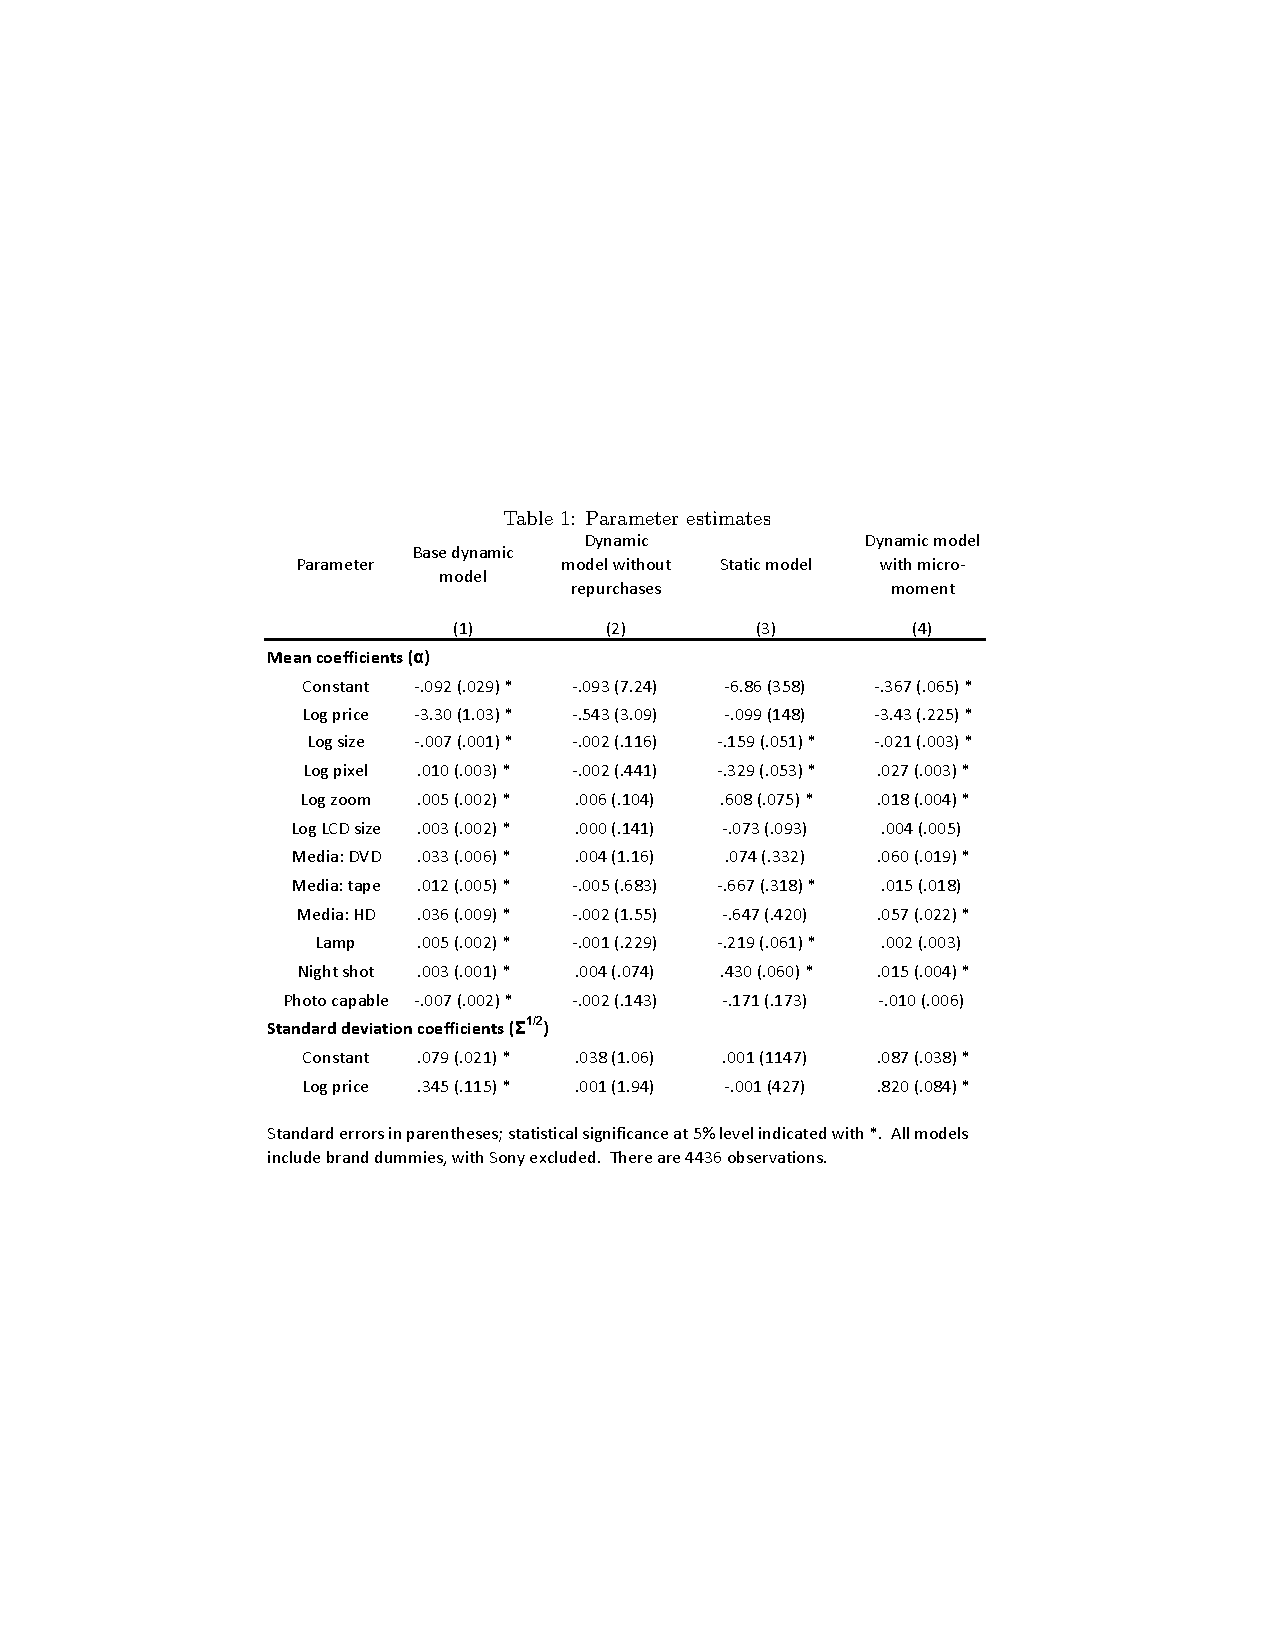
\includegraphics[width=4in]{resources/gandrtable1.pdf}
\end{center}
\end{figure}
\end{frame}

\begin{frame}{G\&R Robustness}
\begin{figure}[htbp]
\begin{center}
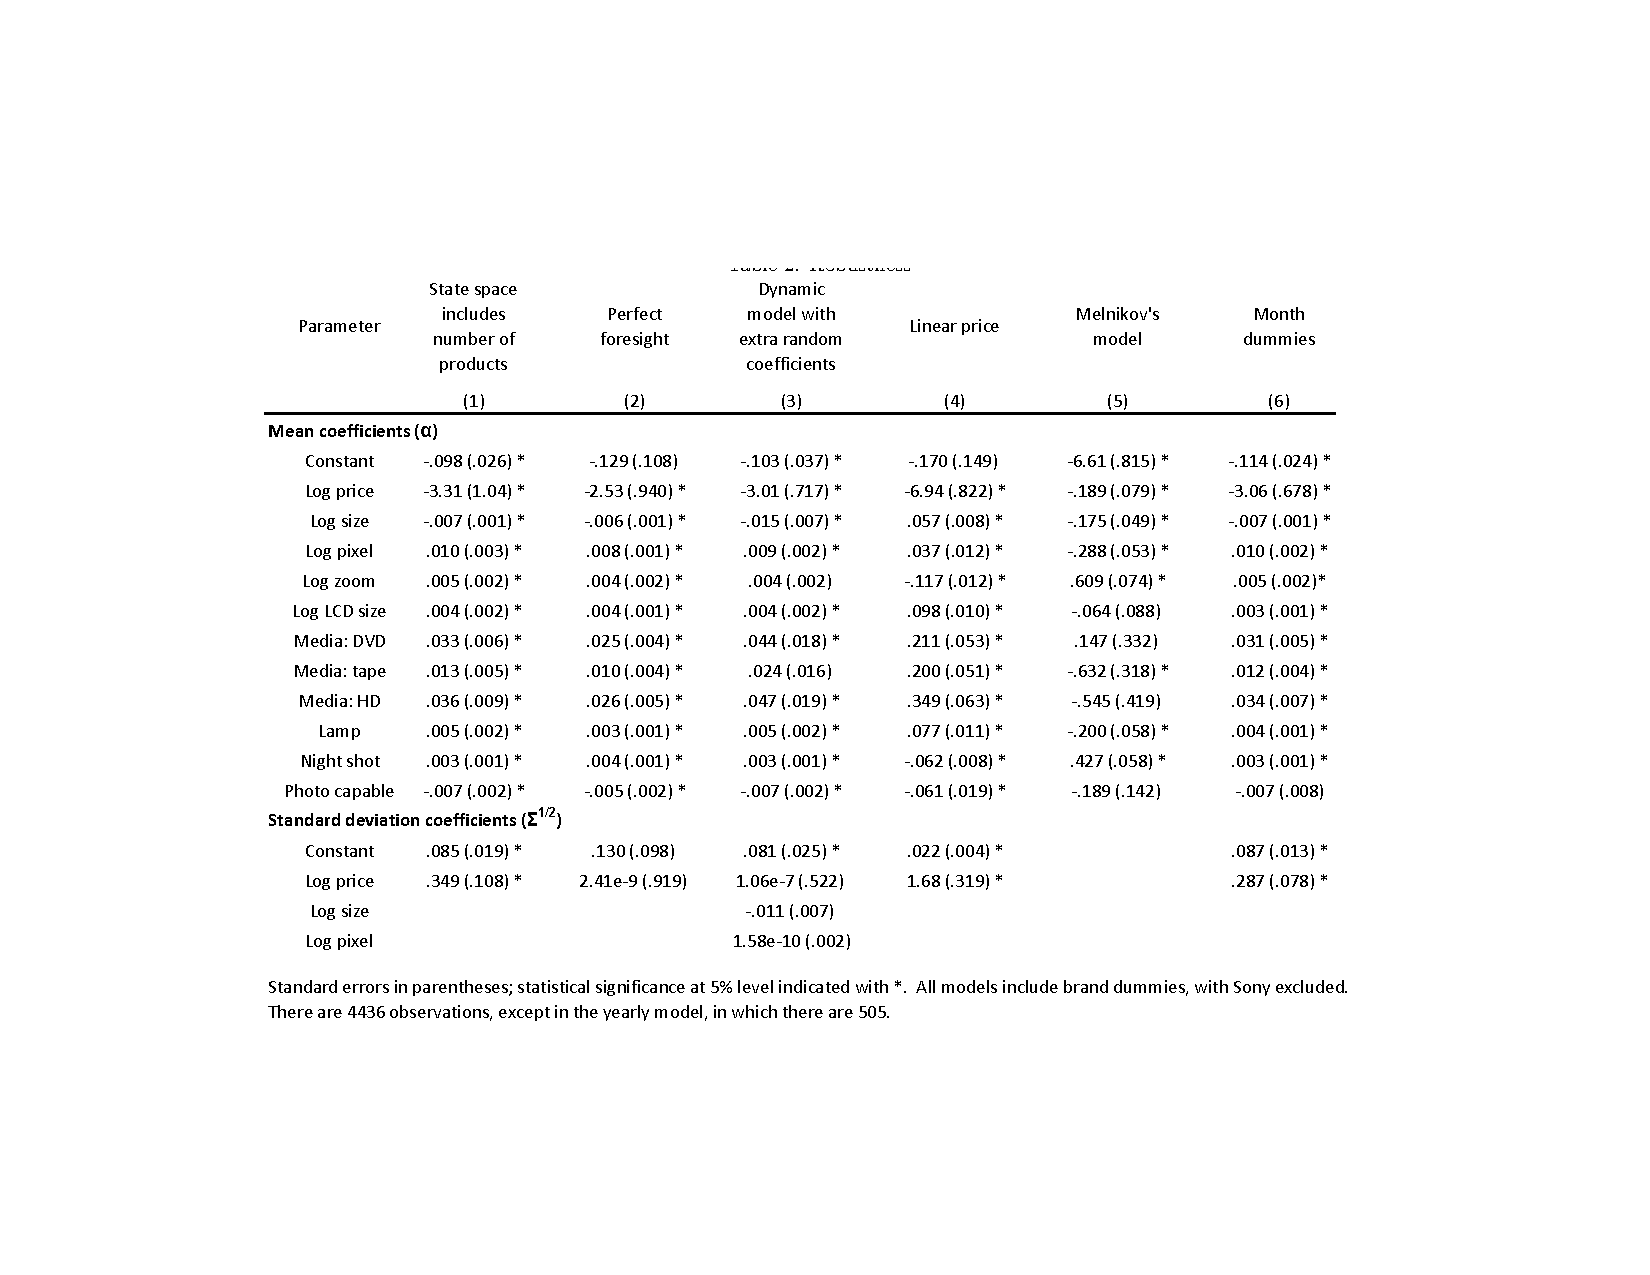
\includegraphics[width=4in]{resources/gandrtable2.pdf}
\end{center}
\end{figure}
\end{frame}


\begin{frame}{Perfect Foresight}
\begin{itemize}
\item Contrary to the static model, price coefficient is negative (as one would expect).
\item Coefficients on many product characteristics are intuitively appealing.
\item Allowing for repeated purchases generates more ``sensible'' results.
\item ``Better results'' from a dynamic model may be due to the fact that people wait to purchase because of the expectations of price declines and not directly because of high prices.
\item Unlike the static model, in dynamic setup the explanation of waiting does not conflict with consumers buying relatively high-priced products.
\item A variety of robustness measures show that the major simplifying assumptions about the dynamics in the model are broadly consistent with the data.
\end{itemize}
\end{frame}

\begin{frame}{Perfect Foresight}
G\&R Report similar elasticities in the perfect foresight case. We make the following simplification
\begin{eqnarray*}
E_{\Omega'}[ EV_i (f_{i0}, \delta_{i,t+1}) |\delta_{i,t}] )] = EV_i (f_{i0}, \delta_{i,t+1})
\end{eqnarray*}
This saves us a lot of headaches:
\begin{itemize}
\item No more integration/interpolation
\item We can solve the problem on the grid!
\item No more belief regressions
\end{itemize}
\end{frame}

\begin{frame}{Conlon (2014)}
Conlon (2014) suggests an alternate formulation of the problem.\\
\vspace{0.25cm}
Assume briefly that there are no upgrades $f_{i0t} = 0$, as well as perfect foresight:
\begin{eqnarray*}
E_{\Omega'}[ EV_i (f_{i0}, \delta_{i,t+1}) |\delta_{i,t}] )] &=& EV_i (f_{i0}, \delta_{i,t+1})  = v_{it} 
\end{eqnarray*}
\begin{eqnarray*}
 v_{it} \equiv EV_i(f_{i0}, \delta_i) &=& \log\left[ \exp( \beta v_{i,t+1})+ \exp(\delta_i)  \right] + \eta \\
\end{eqnarray*}
But we can always add back in the rational expectations error $v_{it} + \alert{\epsilon_{i,t}}$.
\begin{eqnarray*}
s_{ijt} = \int \frac{\exp[x_{jt}\beta + \xi_{jt} ]}{\exp[v_{i,t} + \epsilon_{i,t}] + \sum_k \exp[x_{jt}\beta + \xi_{jt} ]} f(\epsilon_{i,t})
\end{eqnarray*}

\end{frame}

\begin{frame}{The Estimation Problem}
We need to solve $\forall i, t $:
\begin{eqnarray*}
S_{jt}&=& \sum_i w_i s_{ijt}\\
f_{ijt} &=& \overline{\alpha} x_{jt} + \xi_{jt} + \sum_l \sigma_l x_{jl} \nu_{il} \\
s_{ijt} &=& \exp[f_{ijt} - \alpha_i p_{jt} - v_{it} ]\\
v_{it} &=& \log\left[ \exp( \alert{\beta v_{i,t+1}} )+ \exp(\delta_{it})  \right] + \eta\\
\delta_{it}&=& \log \left( \sum_j \exp[ f_{ijt}  -\alpha_i p_{jt} ]  \right)\\
w_{i,t+1} &=& w_{i,t} \left(1-\sum_j s_{ijt} \right)\\
\end{eqnarray*}
Note: that this nests static demand $\alert{\beta} = 0$
\end{frame}

\begin{frame}{Alternative Perspective on Beliefs}
Recall our objective:
\begin{itemize}
\item Plug in an unbiased estimate for the ``no-purchase'' utility.
\item Under perfect foresight this is just the inclusive value of tomorrow's market $\delta_{i,t+1}$  appropriately discounted: $\sum_{k=1}^{T-k} \beta^{t+k} \delta_{i,t+k}$.
\item Different ways to think about \alert{rational expectations}
\begin{itemize}
\item Expectational error of some or all of $\delta_{i,t+k}$'s.
\item Expectational error in today's reservation utility.
\end{itemize}
\end{itemize}
\end{frame}


\begin{frame}{Endogeneity and Instruments}
\begin{itemize}
\item Dynamics mean we  \alert{lean harder on the assumption of exogenous product characteristics} 
\item In one period we can take characteristics as given, but in many periods this becomes less palatable (Do cameras exogenously improve over time?).
\item Endogeneity: price is endogenous while other product characteristics are not, i.e. $x_{jt}$. (Size,Resolution, etc.)
\item Price is chosen by the firms possibly after observing $\xi_{jt}$ and, hence, is endogenous.
\item Instruments: use variables that affect the price-cost margin, e.g. measures of how crowded a product is in characteristics space, which effects price-cost margin and the substitutability across products.
\begin{enumerate}
\item  all of the product characteristics in x;
\item mean product characteristics for a given firm;
\item mean product characteristics for all firms;
\item the count of products offered by the firm and by all firms.
\item changes in costs over time?
\end{enumerate}
\end{itemize}
\end{frame}


\begin{frame}{Hendel and Nevo (2006)}
\begin{itemize}
\item When a supermarket cuts the price of laundry detergent for a week there is a huge increase in sales.
\item This leads us to conclude consumers are extremely elastic with respect to price
\item When a supermarket makes a permanent price cut to laundry detergent, there is little sales impact in the long run.
\item Now consumers look highly inelastic with respect to price
\item Often we use average prices which include high and low periods in regression studies -- does this make sense?
\item How can we resolve this puzzle?
\end{itemize}
\end{frame}

\begin{frame}{Hendel and Nevo (2006)}
\begin{itemize}
\item Hendel and Nevo suggest that consumers respond by temporary price  reductions by stockpiling inventories.
\item Consumers spend down their inventories during periods of high prices
\item Consumers have variable storage costs and price sensitivities. Why?
\item This has implications for inter temporal price discrimination and retail High-Low pricing strategies.
\end{itemize}
\end{frame}

\begin{frame}{Data}
\begin{itemize}
\item 9 Supermarkets in a large midwest city (Dominick's in Chicago)
\item Store-level: for each brand 13 ($j$) size $x$: 32-256oz in each store, each week ($t$)
\begin{enumerate}
\item Price $p_{jxt}$ 
\item Quantity $q_{jxt}$
\item Promotions $a_{jxt}$ (binary for feature/display)
\end{enumerate}
\item Consumers are of type $h$ with utility: $u(c_{ht} + \nu_{ht}; \theta_h)$
\item Current consumption is $c_{ht} = \sum_j c_{jht}$ \alert{not brand specific!}
\item There is a shock affected marginal utility of consumption $\nu_{ht}$.
\item Decision: $d_{hjxt} = 1$ is a purchase of $h$ of brand $j$ and size $x$ at $t$. (includes outside option $=0$).
\end{itemize}
\end{frame}

\begin{frame}{Table 3: Sales}
\begin{figure}[htbp]
\begin{center}
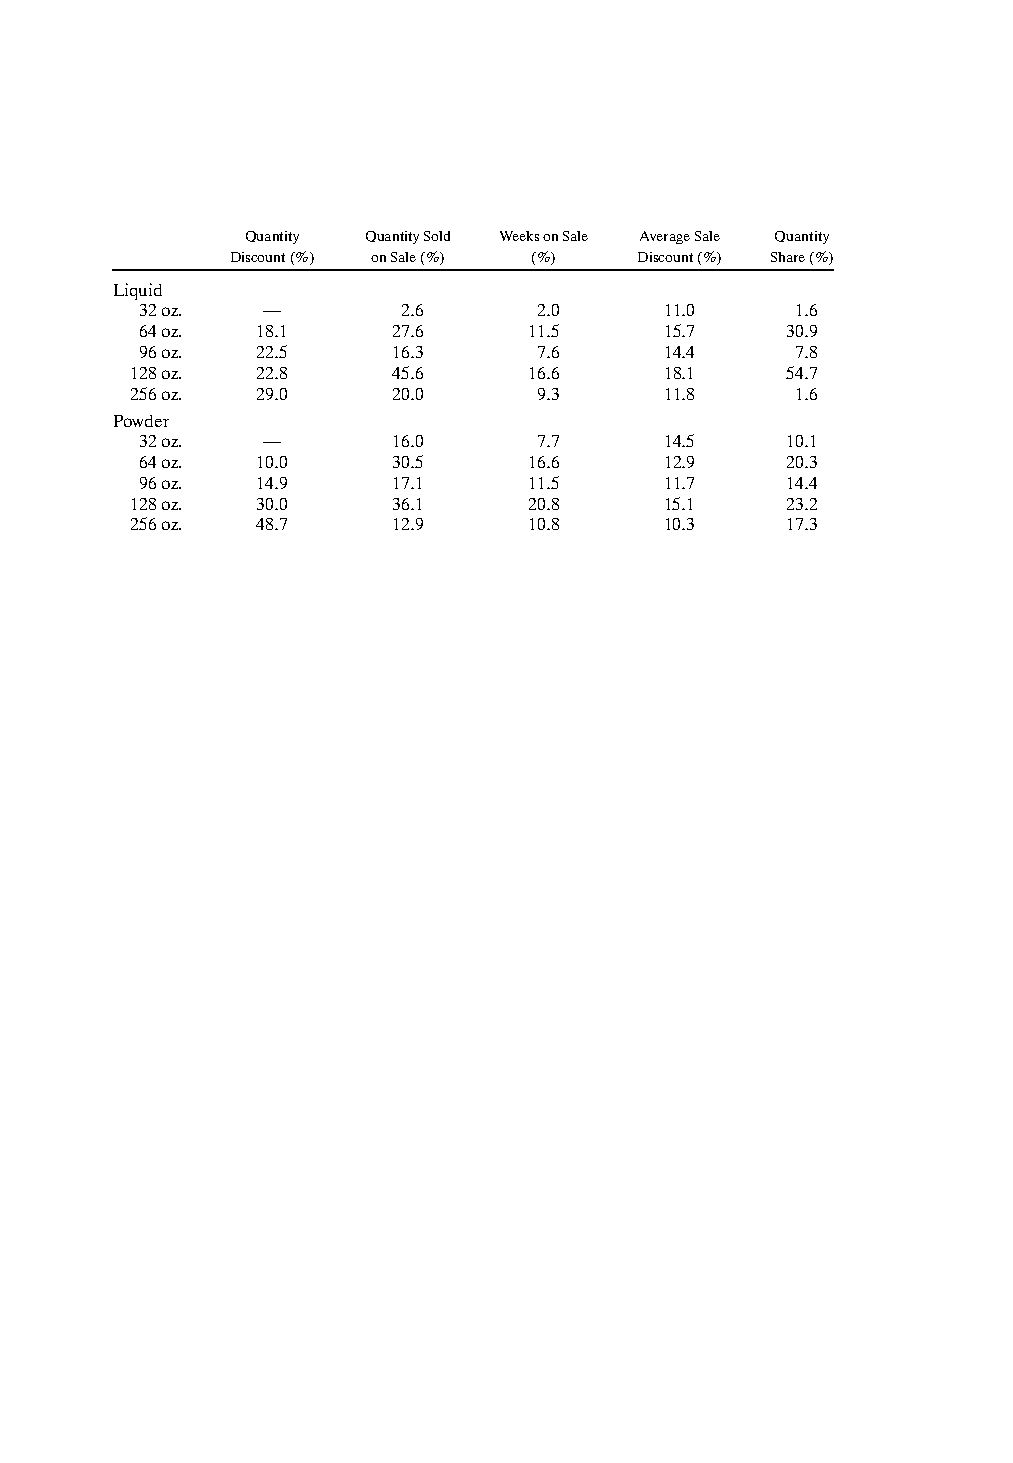
\includegraphics[width=4in]{resources/hntable3.pdf}
\label{gandr1}
\end{center}
\end{figure}
\end{frame}


\begin{frame}{Dynamic Discrete Choice}
\begin{eqnarray*}
V(s_t)&=& \max_{c_h(s_t),d_{jxt}(s_t)} \sum_t \beta^{t-1} E[ u(c_{ht}+\nu_{ht}; \theta_h) - C_h(i_{h,t+1};\theta_h) \\
&+&\sum_j d_{hjxt} (\alpha_h^p p_{jxt} + \xi_{hjx} + \alpha_h^a a_{jxt} + \epsilon_{hjxt} )| s_t]\\
i_{h,t+1} &=& i_{ht} + x_{ht} - c_{ht}\\
\sum_{j,x} d_{hjxt} &=& 1
\end{eqnarray*}
\begin{itemize}
\item Abuse of notation: $x_{ht}$ is size of the choice
\item $C_h(i; \theta_h)$ is cost of storage
\item $s_t$ contains current inventory $i_t$, current prices, and consumption shock $\nu_t$ as well as $\epsilon_{ht}$.
\item $\xi_{jhxt}$ captures expected future differences in utility of $x$ units of $j$ at time of purchase.
\begin{enumerate}
\item as long as discounting is low
\item brand-specific differences in utility (but not consumption) enter linearly.
\end{enumerate}
\end{itemize}
\end{frame}

\begin{frame}{Model Assumptions}
\begin{block}{Assumption 1}
$\nu_t$ is independently distributed over time and across consumers.\\
 \alert{No serial correlation!}
\end{block}
\begin{block}{Assumption 2}
Prices $p_{jxt}$ and advertising $a_{jxt}$ follow an exogenous first-order Markov process.\\
\alert{Hard to justify this with a model of profit maximizing supply!}
\end{block}
\begin{block}{Assumption 3}
$\epsilon_{jxt}$ is i.i.d. extreme value type 1.
\end{block}
\end{frame}

\begin{frame}{Likelihood}
Conditional on Household we can write the probability of a sequence of purchase decisions:
\begin{eqnarray*}
P(d_1,\ldots,d_t | p_1,\ldots,p_T) = \int \prod_t P(d_t | p_t, \\
i_t(d_{t-1},\ldots,d_1, \nu_{t-1},\ldots,\nu_1,i_1))dF(\nu_1,\ldots,\nu_T) dF(i_1)
\end{eqnarray*}
\begin{itemize}
\item Beginning of period inventory depends on previous decisions, previous shocks, and initial inventory.
\item $p_t$ now includes all observed state variables not just prices
\end{itemize}
\end{frame}

\begin{frame}{Choice Problem}
\begin{eqnarray*}
Pr(d_{jx} | p_t,i_t,\nu_t) &=& \frac{\exp[\alpha p_{jxt} + \xi_{jx} + \beta a_{jxt} + M(s_t,j,x)]}{\sum_{k,y} \exp[\alpha p_{kyt} + \xi_{jy} + \beta a_{kyt} + M(s_t,k,y)]}\\
M (s_t,j,x) &=& \max_c [ u(c+\nu_t) - C(i_{t+1}) + \beta E[V(s_{t+1}|d_{jx},c,s_t]]\\
\end{eqnarray*}
\begin{itemize}
\item State space has very high dimension. (Lots of brand-size combos at different prices)
\item Keeping track of all brands/prices would be very costly
\end{itemize}
\end{frame}

\begin{frame}{3-step Procedure}
To reduce complexity, Hendel and Nevo propose a 3-step estimator
\begin{itemize}
\item Maximize likelihood of observed brand choice \alert{conditional} on size in order to recover the $(\alpha,\xi)$ parameters.
\item This avoids solving MDP but instead is just static discrete choice problem (efficiency loss!)
\item Second step: compute \alert{inclusive values} for each size and transition probability matrix.
\item Now solve a quantity choice only nested fixed point problem. The key is that there is \alert{only one ``index price'' per size}.
\item The reason this is feasible is our old friend, the \alert{conditional independence assumption} (of what?)
\end{itemize}
\end{frame}

\begin{frame}{Step 1: Brand Choice}
\begin{eqnarray*}
Pr(d_{jx} | x_t, p_t,i_t,\nu_t) &=& \frac{\exp[\alpha^p p_{jxt} + \xi_{jx} + \alpha^a a_{jxt}]}{\sum_{k,y} \exp[\alpha^p p_{kyt} + \xi_{jy} + \alpha^a a_{kyt}  ] }\\
&=&Pr(d_{jx} | x_t, p_t)
\end{eqnarray*}
\begin{itemize}
\item The trick is that $M(s_t,j,x)$ is the same for all products of the same size $x$.
\item This means the dynamics drop out of the brand-choice equation conditional on $x_t$.
\item We can recover $(\alpha, \xi)$ from static demand estimation!
\end{itemize}
\end{frame}

\begin{frame}{Step 2: Inclusive Values}
\begin{eqnarray*}
\omega_{xt} &=& \log \left( \sum_k \exp(\alpha^p p_{kxt} + \xi_{xt} + \alpha^a a_{kxt}) \right)
\end{eqnarray*}
\vspace{-0.5cm}
\begin{block}{Assumption 4: IVS}
$$F(\omega_t | s_{t-1}) = F(\omega_t | \omega_{t-1})$$
\end{block}
\begin{itemize}
\item Compute ex-ante expected utility of purchasing size $x$ in period $t$
\item Does not depend on which $j$ is purchased.
\item IVS means we can keep track of a lot less information!
\item Same as G\&R two price vectors with same inclusive values must have same transition probabilities.
\item Do individual prices still matter? (Test)
\end{itemize}
\end{frame}


\begin{frame}{Step 3: Dynamic Choice of Size}
\begin{eqnarray*}
V(i,\omega_t,\epsilon_t,\nu_t) = \max_{c,x} [ u(c + \nu_t) - C(i_{t+1}) + \omega_{xt} + \epsilon_{xt} + \\
\beta E[V(i_{t+1},\omega_{t+1},\epsilon_{t+1},\nu_{t+1}) | i_t, \omega_t, \epsilon_t, \nu_t, c, x] ]
\end{eqnarray*}

\begin{itemize}
\item Compute ex-ante expected utility of purchasing size $x$ in period $t$
\item Does not depend on which $j$ is purchased.
\item IVS means we can keep track of a lot less information!
\item Same as G\&R two price vectors with same inclusive values must have same transition probabilities.
\item Do individual prices still matter? (Test)
\end{itemize}
\end{frame}

\begin{frame}{Key Proposition}
How do we know that the simplified problem has the same solution as the original dynamic problem?
\begin{eqnarray*}
P(x_t | i_t,p_t, \nu_t) = P(x_t | i_t, \omega(p_t),\nu_t)
\end{eqnarray*}

\begin{itemize}
\item Before we got to see the entire state $s_t$
\item Now we only see the expected utility of $x_t$ aka $\omega_{xt}$
\item The proof relies on Assumption 3(IID Logit errors) and Assumption 4 (IVS).
\end{itemize}
\end{frame}

\begin{frame}{Computational Details}
Iterate policy evaluation and policy improvement 
\begin{enumerate}
\item Approximate the value function by a polynomial function of $s_t$. (Logarithmic)
\item Guess an optimal policy and minimized (LSQ) deviation between the value function and expected future value
\item Update the policy function for every state
\item Update expectation with coefficients and expected value of state variables
\item Repeat until value function coefficients converge
\end{enumerate}
This is a \alert{Smooth Approximation} approach
\end{frame}


\begin{frame}{Table 4: Brand Choice Estimates}
\begin{figure}[htbp]
\begin{center}
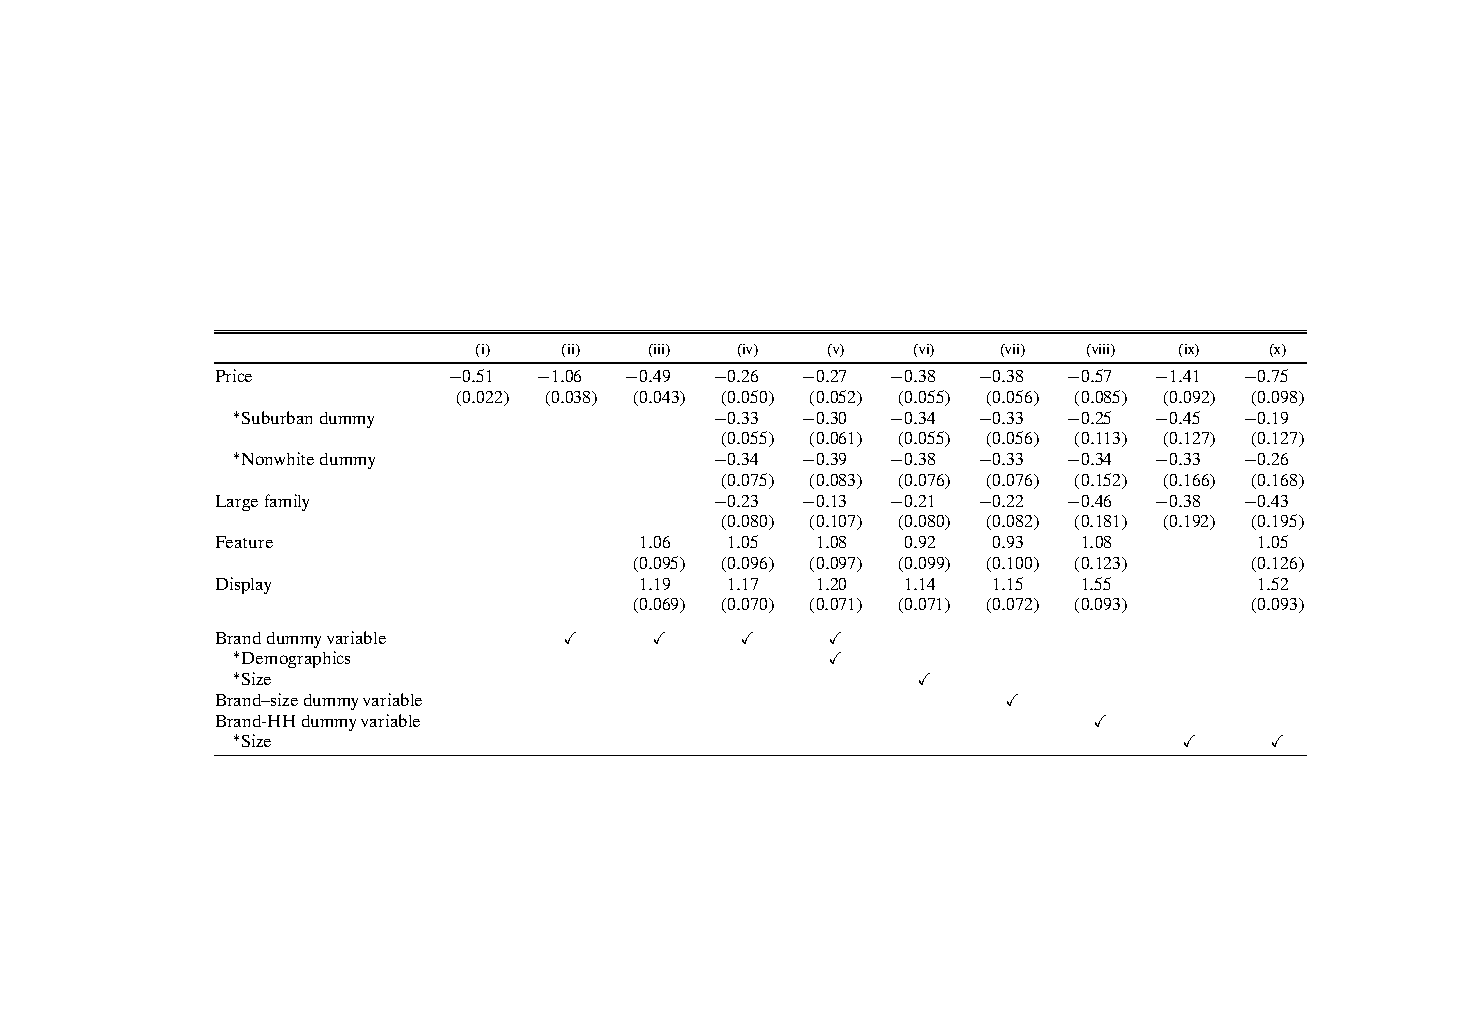
\includegraphics[width=4in]{resources/hntable4.pdf}
\label{gandr1}
\end{center}
\end{figure}
\end{frame}

\begin{frame}{Table 5: Belief Process Estimates}
\begin{figure}[htbp]
\begin{center}
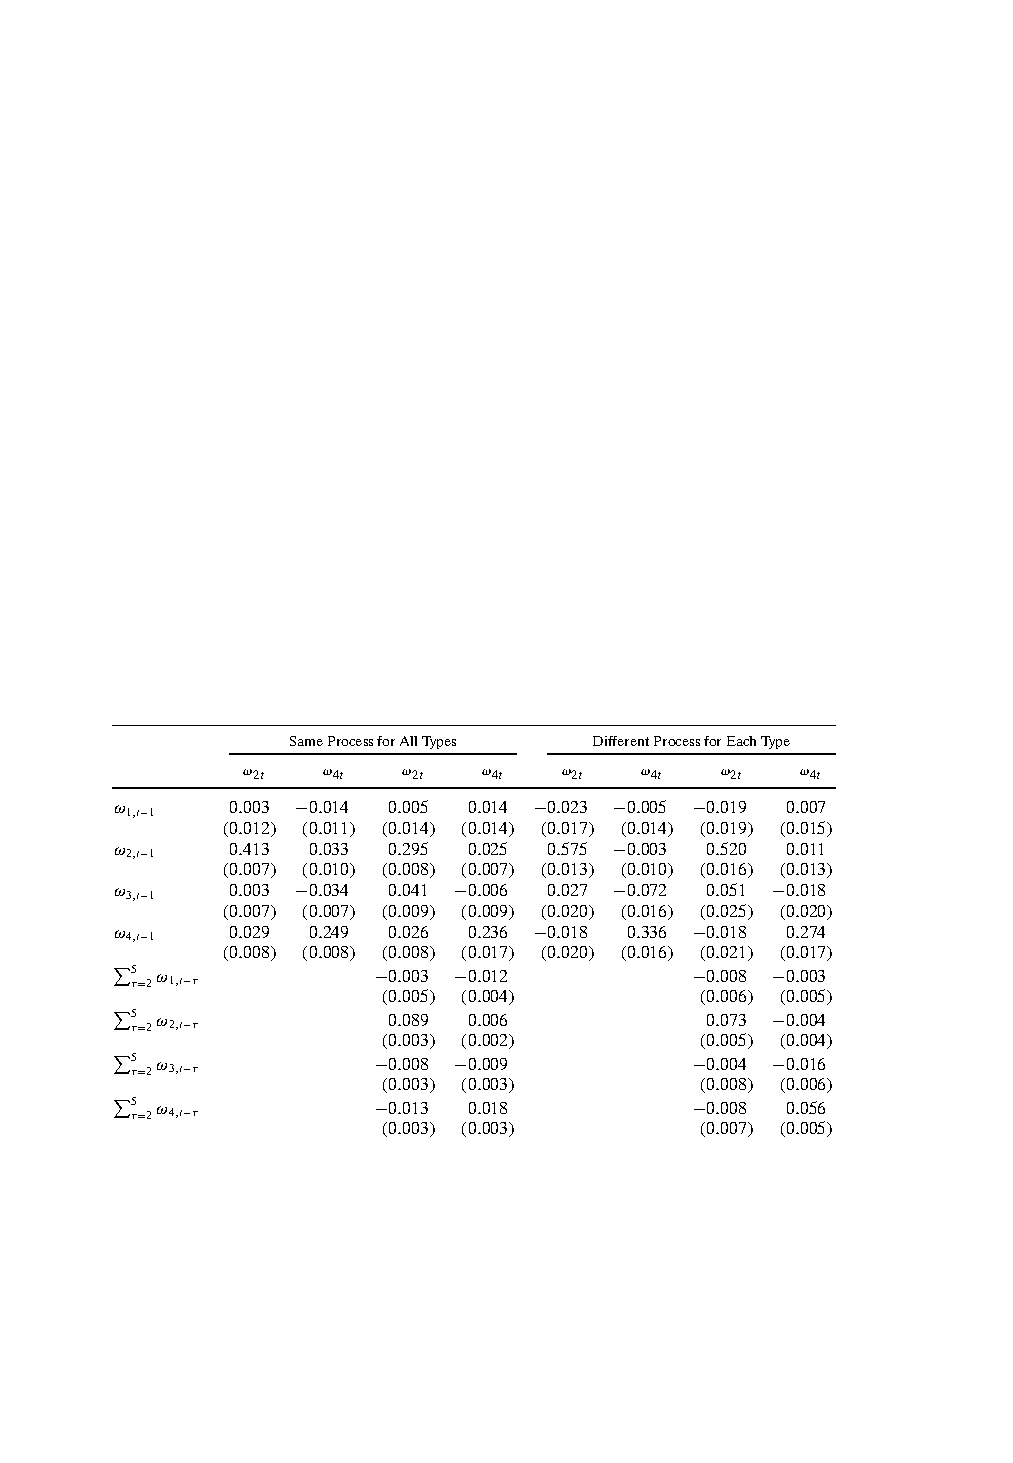
\includegraphics[width=4in]{resources/hntable5.pdf}
\label{gandr1}
\end{center}
\end{figure}
\end{frame}

\begin{frame}{Table 5: Dynamic Problem Estimates}
\begin{figure}[htbp]
\begin{center}
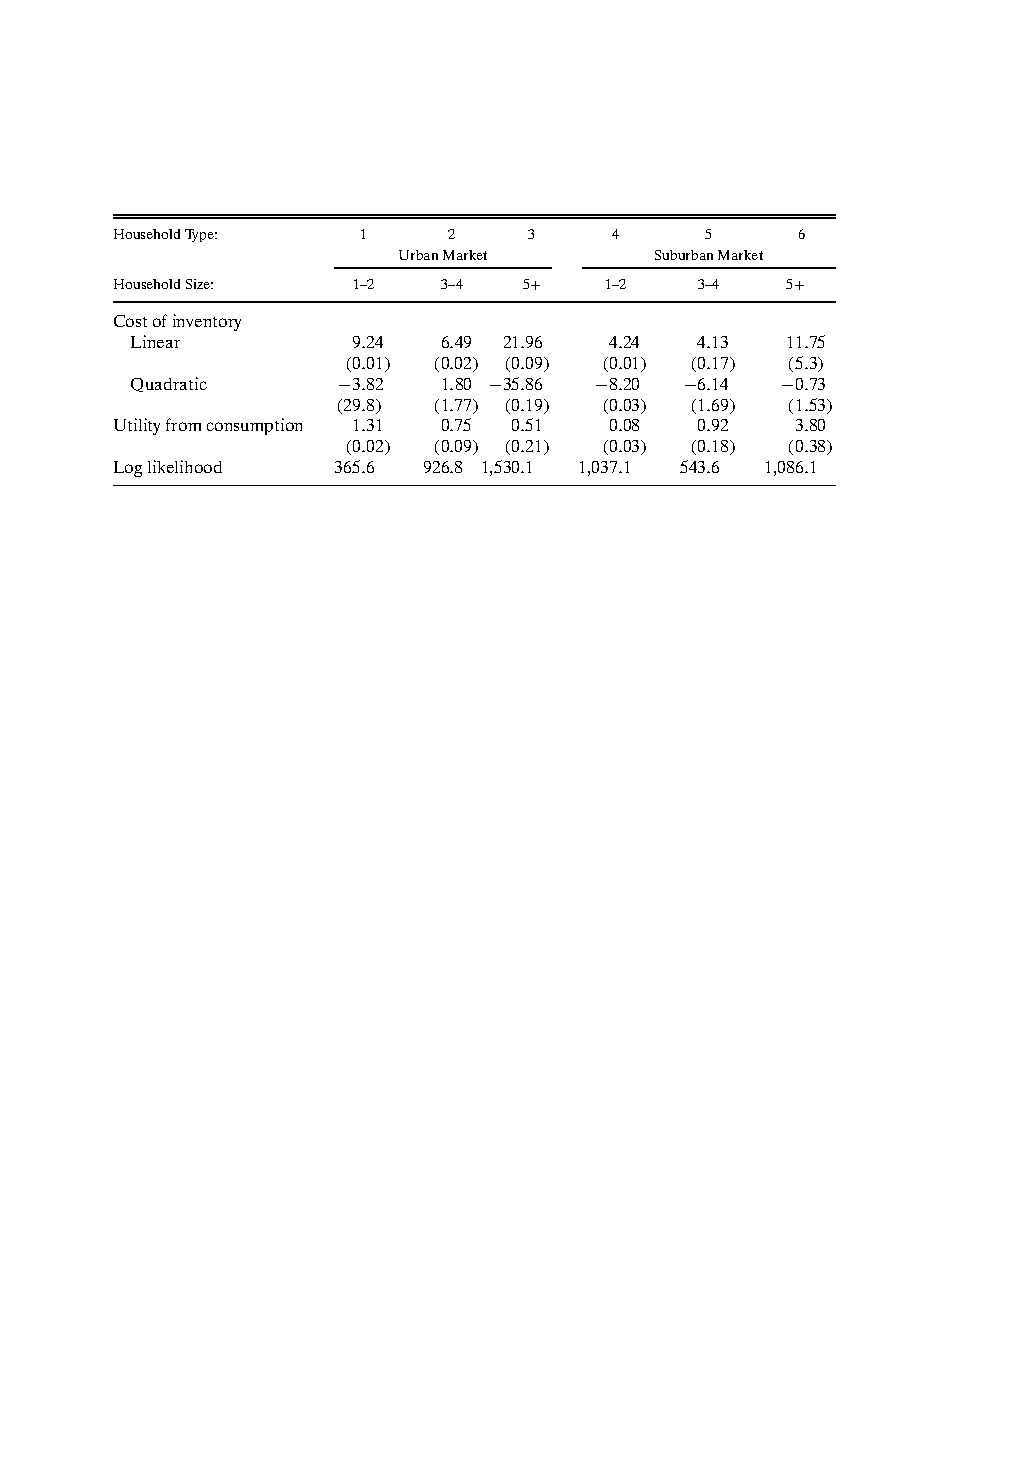
\includegraphics[width=4in]{resources/hntable6.pdf}
\label{gandr1}
\end{center}
\end{figure}
\end{frame}

\begin{frame}{Table 8: Elasticities Compared to Static Model}
\begin{figure}[htbp]
\begin{center}
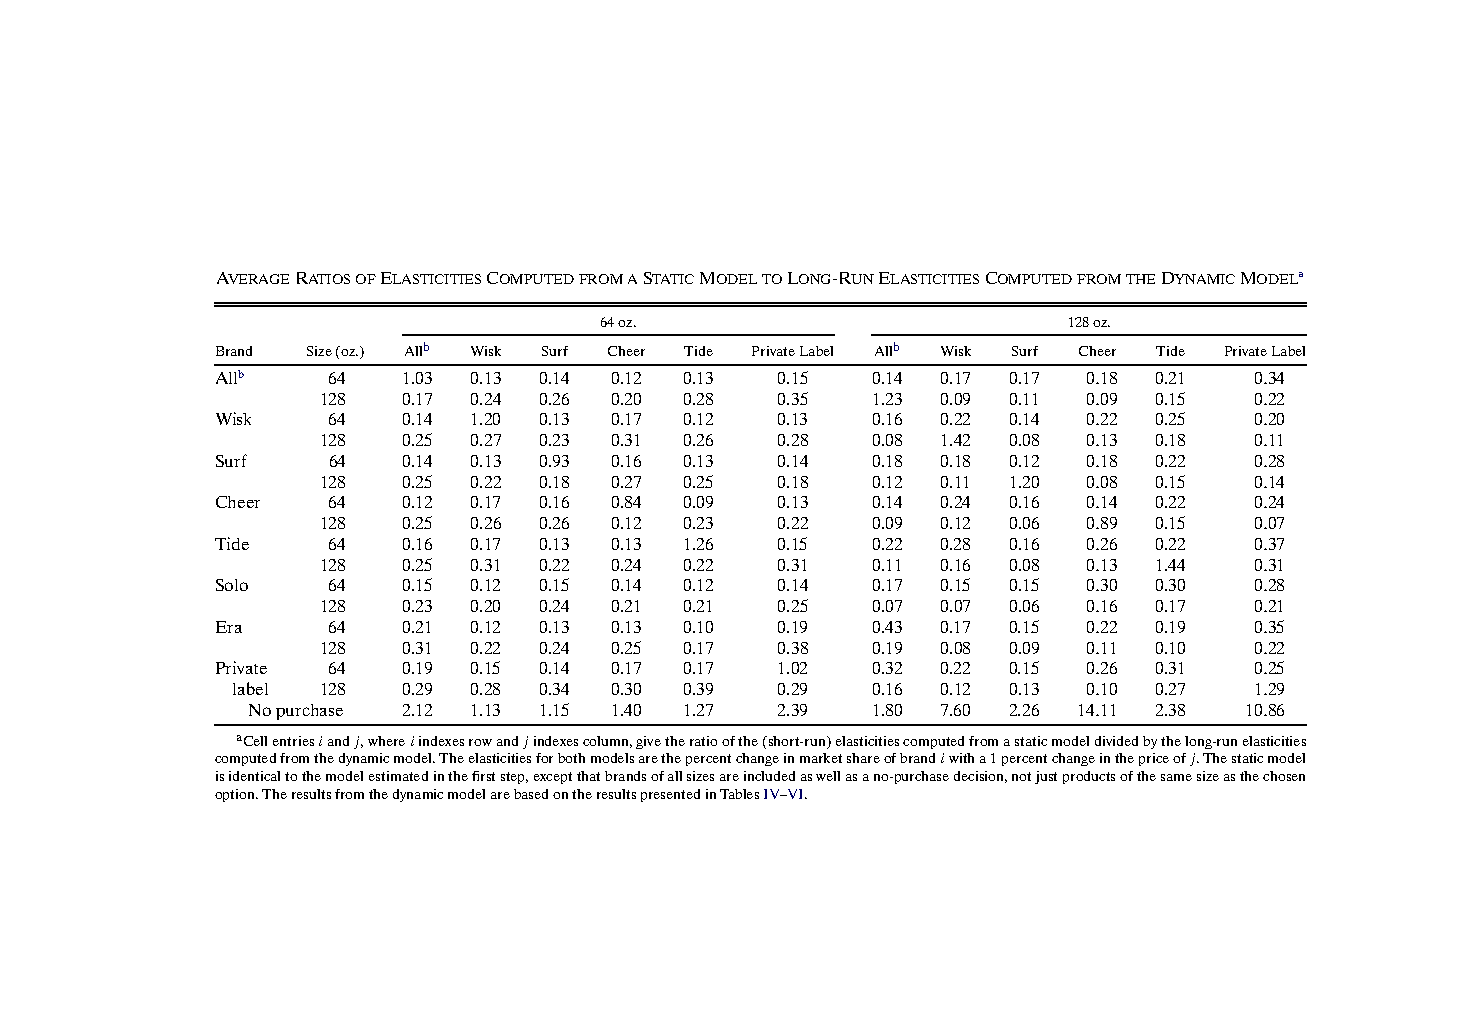
\includegraphics[width=4in]{resources/hntable8.pdf}
\label{gandr1}
\end{center}
\end{figure}
\end{frame}

%
%\begin{frame}{The Estimation Problem}
%We need to solve $\forall i, t $:
%\begin{eqnarray*}
%S_{jt}(\theta) &=& \sum_i w_i s_{ijt}(f_{i0t},\delta_{it})\\
%f_{ijt} &=& \overline{\alpha}^x x_{jt} + \xi_{jt} + \sum_l \sigma_l x_{jl} \nu_{il} \\
%s_{ijt} &=& \frac{\exp[f_{ijt} - \alpha_i p_{jt} + \beta v_{i,t+1}] }{\exp [v_{it} ]}\\
%v_{i,t} &=& \log\left[ \alert{\exp(\beta v_{i,t+1})} + \exp(\delta_i)  \right]\\
%\delta_{it} &=& \log \left( \sum_j \exp[ f_{ijt}  -\alpha_i p_{jt} +\alert{\beta  v_{i,t+1}}]  \right)\\
%w_{i,t+1} &=&h(w_{i,t},s_{ijt})
%\end{eqnarray*}
%The only difference between this and BLP (in red).
%\end{frame}
%

%\begin{frame}{The Estimation Problem}
%We need to solve $\forall i, t $:
%\begin{eqnarray*}
%s_{ijt} &=& \exp[f_{ijt} - \alpha_i p_{jt} + \beta v_{i,t+1} - v_{i,t}] \\
%v_{i,t} &=& \log\left[ \alert{\exp(\beta v_{i,t+1})} + \exp(\delta_{it})  \right]\\
%\delta_{it} &=& \log \left( \sum_j \exp[ f_{ijt}  -\alpha_i p_{jt} +\alert{\beta  v_{i,t+1}}]  \right)\\
%\exp[v_{i,t} - \beta v_{i,t+1}] &=& \frac{ \exp(\beta v_{i,t+1})+ \exp(\delta_{it})} {\exp[\beta v_{i,t+1}]} \\
%&=& 1 + \exp{\delta_{it} - 
%\end{eqnarray*}
%\end{frame}

%\begin{frame}
%\frametitle{Adoption Problem}
%We'll begin by considering an adoption problem.
%\begin{itemize}
%\item Consumers make only one purchase decision
%\item Now we don't need to keep track of flow utilities in every period \alert{because you never purchase again}.
%\item Problem becomes an \textit{optimal stopping problem}
%\item Only keep track of value function for consumers with no durable.
%\item If consumers know future characteristics of products including $\epsilon_{ijt}$ then this is just a $J \times T$ static problem.
%\end{itemize}
%\vspace{0.5cm}
%We can assume that consumers receive PDV of entire future stream of utility payments $u_{i0t}$ when they make a purchase.
%\begin{eqnarray*}
%V_i(u_{i0t},\varepsilon_{i t}, \Omega_t) &=& 
%&& \max_j \underbrace{u_{ijt} + \beta E_{\Omega}[ E_{\varepsilon} V_i ( \varepsilon_{it}, \Omega_{t+1}) |\Omega_{t} ]  \}}_{\tilde{u}_{ijt}}
%\end{eqnarray*}
%\end{frame}

%
%\begin{frame}
%\frametitle{Solving the Adoption Problem}
%\begin{itemize}
%\item It is now impossible for $\overline{u}_{i0t}$ to change over time except through $\varepsilon_{i0t}$.
%\item And since $\tilde{u}_{ijt}$ is all paid at once we might as well normalize $\overline{u}_{i0t} = 0$.
%\item[�]
%� Helpful to write: $EV_i(\Omega_t)= \int V_i(\varepsilon_{it},  \Omega_t)f(\varepsilon)$ \alert{Rust's Trick}
%\end{itemize}
%\begin{eqnarray*}
%V_i(u_{i0t},\varepsilon_{i t}, \Omega_t) &=& \max \{ u_{i0t} + \beta E[ E_{\varepsilon} V_i (u_{i0t}, \varepsilon_{it}, \Omega_{t+1}) |\Omega_{t} ] , \max_j \alert{\tilde{u}_{ijt}} \}
% \\
% &=& \max \{\beta E_{\Omega}[ EV_i(\Omega_{t+1}) |\Omega_{t} ] +\varepsilon_{i0t}, \max_j \tilde{u}_{ijt} \}
% \end{eqnarray*}
% \vspace{-0.5cm}
%\end{frame}
%
%
%
%\begin{frame}
%\frametitle{Logit Inclusive Value Trick}
%The $E_{\varepsilon}[ \max_j \tilde{u}_{ijt}]$ has a closed form expression based on the logit inclusive value:
%\begin{eqnarray*}
%\delta_{it} = E_{\varepsilon}[\max_j \tilde{u}_{ijt} ] &=& \log \sum_j \exp(x_{jt} \alpha_i^x - \alpha_{i}^p p_{jt} +  \xi_{jt})\\
%EV_i(\Omega_t)&=& \max \{\beta E_{\Omega}[ EV_i(\Omega_{t+1}) |\Omega_{t} ] +\varepsilon_{i0t}, \max_j \tilde{u}_{ijt} \}\\
%&=& \max \{\beta E_{\Omega}[ EV_i(\Omega_{t+1}) |\Omega_{t} ] +\varepsilon_{i0t}, \delta_{it} \}\\
%&=& \log \left( \exp[\beta E_{\Omega}[ EV_i(\Omega_{t+1}) |\Omega_{t} ] +  \exp[\delta_{it}] \right) + \eta
% \end{eqnarray*}
%Where $\eta = 0.577215665$ (Euler's Constant).
%\end{frame}
%
%\begin{frame}
%\frametitle{Inclusive Value Sufficiency}
%\begin{eqnarray*}
%EV_i(\Omega_t) &=& \log \left( \exp[\beta E_{\Omega}[ EV_i(\Omega_{t+1}) |\Omega_{t} ] +  \exp[\delta_{it}] \right) + \eta
% \end{eqnarray*}
%The fact that the expected value function depends recursively on itself and $\delta_{it}$ (Inclusive Value) leads to the following assumption.
%\begin{block}{Inclusive Value Sufficiency}
%If $\delta(\Omega) = \delta(\tilde{\Omega})$ then $g(\delta(\Omega') | \Omega)= g(\delta(\tilde{\Omega'}) | \tilde{\Omega})$
%\end{block}
%\end{frame}
%

\end{document}













































